\documentclass{article}
\usepackage[utf8]{inputenc}
\usepackage[ruled,vlined]{algorithm2e}
\usepackage{listings}
\usepackage{xcolor}
\usepackage{graphicx}
\usepackage{siunitx}
\usepackage{amsfonts}

\newcommand{\R}{\mathbb{R}}

\author{Benamara Abdelkader \\ Benichou Yaniv }
\date{08 Juin 2020}

\begin{document}
\title{Projet maths-info \\ 
Résolution d'équations non-linéaires}
\maketitle

\newpage
\tableofcontents
\newpage

\section{Introduction}
    Le but de ce projet est de décrire les algorithmes les plus fréquemment utilisés pour résoudre des équations non linéaires du type : \\ f(x) = 0
                         
\newpage


\section{Méthode De Dichotomie}
\subsection{Théoreme des valeurs intermédiaires :}
Pour toute application continue $ f : [a, b] \to \R $ et tout reel u compris entre f(a) et f(b), il existe au moins un reel c compris entre a et b tel que f(c) = u. \\
En particulier on a la version de Bolzano qui nous interesse précisement.

\subsection{Théoreme de Bolzano}
Soit une fonction continue $ f : [a, b] \to \R $ \\
si $ f(a)f(b) < 0 $  alors $ \exists \alpha \in  ]a, b[ $ tel que f($\alpha$)=0. \\ 


On considère deux nombres réels a et b et une fonction réelle f continue sur l'intervalle [a, b] telle que f(a) et f(b) soient de signes opposés. Supposons que nous voulions résoudre l'équation f(x) = 0. D'après le théorème des valeurs intermédiaires, f a au moins un zéro dans l’intervalle [a, b]. La méthode de dichotomie consiste à diviser l’intervalle en deux en calculant m = (a+b) / 2. \\
Il y a maintenant deux possibilités : ou f(a) et f(m) sont de signes contraires, ou f(m) et f(b) sont de signes contraires.

L’algorithme de dichotomie est alors appliqué au sous-intervalle dans lequel le changement de signe se produit, ce qui signifie que l’algorithme de dichotomie est récursif.
\subsection{L'algorithme de dichotomie}

\begin{algorithm}[H]
\SetAlgoLined
\KwResult{millieu $\:$ tq $\:$ f(millieu)=0}
 initialization\;
 \While{fin-debut > err}{
  millieu = (debut + fin ) / 2\;
  \eIf{f(millieu) >  0}{
   fin = millieu\;
   }{
   debut=millieu\;
  }
 }
 \caption{Méthode de dichotomie}
\end{algorithm}

\definecolor{codegreen}{rgb}{0,0.6,0}
\definecolor{codegray}{rgb}{0.5,0.5,0.5}
\definecolor{codepurple}{rgb}{0.58,0,0.82}
\definecolor{backcolour}{rgb}{0.95,0.95,0.92}

\lstdefinestyle{mystyle}{
    backgroundcolor=\color{backcolour},   
    commentstyle=\color{codegreen},
    keywordstyle=\color{magenta},
    numberstyle=\tiny\color{codegray},
    stringstyle=\color{codepurple},
    basicstyle=\ttfamily\footnotesize,
    breakatwhitespace=false,         
    breaklines=true,                 
    captionpos=b,                    
    keepspaces=true,                 
    numbers=left,                    
    numbersep=5pt,                  
    showspaces=false,                
    showstringspaces=false,
    showtabs=false,                  
    tabsize=2
}
\lstset{style=mystyle}
\newpage
\begin{lstlisting}[language=Python, caption=Méthode de dichotomie en Python]
class Dichotomie(Equa_Solver):

    def solve(self):
        # Donnees en parametres
        a , b = self.a , self.b
        err=self.err
        try:
            f = lambda x: eval(str(self.f))
        except (TypeError,SyntaxError):
            return
        x_list=[]

        print(f" Fonction   : {self.f}")
        print(f" Intervalle : [{a},{b}]")
        print(f" Erreur     : {err} \n")


        if( f(a)*f(b) > 0):
            raise SolverException(" f(a) et f(b) doivent etre de signe different !")

        else:
            debut = a
            fin = b
            n=1

            while (fin - debut > err):
                millieu = (debut + fin) / 2
                x_list.append(millieu)
                print(f"Found solution after {n} iterations : {millieu} ")
                n+=1
                if (f(debut) * f(millieu) < 0):
                    fin = millieu
                else:
                    debut = millieu

            print(f" Solution approchee de f(x) = 0 est : {millieu}\n")
            return x_list
\end{lstlisting}








\newpage




\section{Méthode de Newton}
\subsection{Présentation} 
\quad Afin de mettre au point des algorithmes possédant de meilleures propriétés de convergence que la méthode de dichotomie, il est nécessaire de prendre en
compte les informations données par les valeurs de f et, éventuellement, par sa dérivée f' (si f est différentiable) ou par une approximation convenable de celle-ci.\\
 L'algorithme de la méthode de Newton peut être présenté brièvement comme suit: à chaque itération, la fonction dont on cherche un zéro est linéarisée en l'itéré (ou point) courant et l'itéré suivant est pris égal au zéro de la fonction linéarisée. Cette description sommaire indique qu'au moins deux conditions sont requises pour la bonne marche de l'algorithme : la fonction doit être différentiable aux points visités (pour pouvoir y linéariser la fonction) et les dérivées ne doivent pas s'y annuler (pour que la fonction linéarisée ait un zéro) ; s'ajoute à ces conditions la contrainte forte de devoir prendre le premier itéré assez proche d'un zéro régulier de la fonction (i.e., en lequel la dérivée de la fonction ne s'annule pas), pour que la convergence du processus soit assurée. \\


Ecrivons pour cela le développement de Taylor de f en $\alpha$  au premier ordre.
On obtient alors la version linéarisée du problème
$f(\alpha) = 0 = f(x) + (\alpha−x)f(\eta)$,
où $\eta$ est entre $\alpha$ et x. L’équation  conduit à la méthode itérative suivante :
$\forall k \geq 0$, étant donné $x^k$ , déterminer $x^(k+1)$ en résolvant l’équation
$ f(x^k) + (x^{k+1}-x^k)q_k = 0$, où $q_k$ est une approximation de $f(x^k)$.

\quadd Considérons maintenant quatre choix particuliers de $q_k$ . \\
\quadd Ici on pose : \quad $q_k=f'(x_k)  \quad \forall k\geq 0$ \\ et en se donnant la valeur initiale $x^0$ , on obtient la méthode de Newton : \\
    \quadd $x^{k+1} = x^k - \frac{f(x^k)}{f'(x^k)} \quad \forall k\geq 0$ \\

A la k-ème itération, la méthode de Newton nécessite l’évaluation des deux fonctions f et f' au point $x^k$. Cet effort de calcul supplémentaire est plus
que compensé par une accélération de la convergence, la méthode de Newton étant d’ordre 2. 

Or, il est possible que la dérivée de la fonction f soit relativement pénible à calculer et c'est pour ça que nous avons présenté une deuxieme version d'implémentation de cette méthode,sans dérivée donnée en paramètre,puisqu'elle est automatiquement calculée.
Cela rend la méthode de Newton très agréble à utiliser,puisqu'elle converge très rapidement et ne nécessite donc, uniquement un point approximatif $x_0$ comme argument supplementaire à la fonction.


\subsection{Interpretation Géometrique}
La méthode qu’on vient de décrire revient à chercher l’intersection entre
l’axe des x et la droite de pente $q_k$ passant par le point ($x^k$,$f(x^k)$),ce qui s’écrit
$x^{k+1} = x^k−q_k − 1 f(x^k) ) \forall k \geq 0 $.
\subsection{Implementation du code}
\begin{lstlisting}[language=Python, caption=Méthode de Newton en Python]

class Newton(Equa_Solver):

    def solve_with_df(self):
        f=self.f
        Df=self.df
        max_iter=self.max_iter
        x0=self.x0
        epsilon=self.err
        x_list=[]

        fx = lambda x: eval(str(f))
        dfx = lambda x: eval(str(Df))
        print("\n\nfunction f : ", f, "\n", "Derivative f' : ", Df, "\n", "--------------------------------")
        xn = x0
        for n in range(0, max_iter):
            fxn = fx(xn)
            x_list.append(xn)
            self.affiche_info(n,xn,fxn)
            if abs(fxn) < epsilon:
                print('Found solution after', n, 'iterations.')
                print("the approximate solution is : ",x_list[-1])
                return x_list

            Dfxn = dfx(xn)

            if Dfxn == 0:
                print('Zero derivative. No solution found.')
                return None
            xn = xn - fxn / Dfxn

        print('Exceeded maximum iterations. No solution found.')
        return None
        
    def solve_without_df(self):
        f=self.f
        max_iter=self.max_iter
        x0=self.x0
        epsilon=self.err
        x_list=[]


        x = Symbol('x')
        fx = lambda x: eval(str(f))
        dfx = lambda x: eval(str(diff(f)))
        print("\n\nfunction f : ", f, "\n", "Derivative f' : ", diff(f), "\n", "--------------------------------")

        xn = x0

        for n in range(0, max_iter):
            fxn = fx(xn)
            x_list.append(xn)
            self.affiche_info(n, xn, fxn)
            if abs(fxn) < epsilon:
                print('Found solution after', n, 'iterations.')
                print("the approximate solution is : ",x_list[-1])
                return x_list
                
            Dfxn = dfx(xn)
            if Dfxn == 0:
                print('Zero derivative. No solution found.')
                return None
            xn = xn - fxn / Dfxn
        print('Exceeded maximum iterations. No solution found.')
        return None
\end{lstlisting}
\newpage
\subsection{Convergence}

Avantages de la méthode : s’il y a convergence, celle-ci est rapide (souvent quadratique), elle nécessite un
seul point de départ.

Inconvénients de la méthode : f doit être suffisamment régulière, la convergence n’est pas assurée dans tous
les cas, s’il y a plusieurs racines elle ne converge par forcément vers la plus proche du point de départ.





\newpage
\section{Méthode des Cordes}
\subsection{Présentation} 
La méthode des cordes est une méthode comparable à celle de Newton, où l'on remplace ${\displaystyle f'(x_{n})\,}, par \quad  {\displaystyle {\frac {f(x_{n})-f(x_{n-1})}{x_{n}-x_{n-1}}}}$ \\ \\
L'initialisation nécessite deux points $x_0$ et $x_1$, proches, si possible, de la solution recherchée. Il n'est pas nécessaire que $x_0$ et $x_1$ encadrent une racine de f. La méthode des cordes peut aussi être vue comme une généralisation de la méthode de la fausse position, où les calculs sont itérés. \\
 Ici on pose donc : $q_k = \frac{f(x^k) - f(x^{k-1})}{x^k - x^{k-1}} \quad \forall k \geq 0 $
 d’où on déduit, en se donnant deux valeurs initiales $x^{−1}$ et $x^0$,la relation suivante : \\ \\
    $x^{k+1} = x^k - \frac{x^k - x^{k-1}}{ f(x^k)- f(x^{k-1}) }f(x^k)$

\subsection{Interpretation Géometrique}
\subsection{Implementation du code}
\begin{lstlisting}[language=Python, caption=Méthode des cordes en Python]
    class Cordes(Equa_Solver):
    
    def solve(self):
        f=self.f
        a,b =self.a,self.b
        max_iter=self.max_iter
        epsilon=self.err
        x_list=[]

        fx = lambda x: eval(str(f))
        print("\n\nfunction f : ", f, " dans l'intervalle [", a, ",", b, "] \n", "--------------------------------")


        for n in range(0, max_iter):
            self.affiche_info(n, b, fx(b))
            x_list.append(b)
            if (abs(a - b) < epsilon):
                print('Found solution after', n, 'iterations.')
                return x_list

            z = (a * fx(b) - b * fx(a)) / (fx(b) - fx(a))
            a, b = b, z

        print('Exceeded maximum iterations =', max_iter, '.No solution found.')
        return None
\end{lstlisting}
\newpage
\subsection{Convergence}
Si les valeurs initiales x0 et x1 sont suffisamment proches de la solution, la méthode aura un ordre de convergence de

${\displaystyle \varphi ={\frac {1+{\sqrt {5}}}{2}}\simeq 1,618} $ qui est le nombre d'or.






\newpage
\section{Méthode de la Fausse-Position}
\subsection{Présentation} 
    

\subsection{Interpretation Géometrique}
\subsection{Implementation du code}
\begin{lstlisting}[language=Python, caption=Méthode de la Fausse Position en Python]
class FalsePosition(Equa_Solver):

    def solve(self):
        f=self.f
        a,b=self.a,self.b
        tol=self.err
        x_list=[]
        fx = lambda x: eval(str(f))
        print("\n\nfunction f : ", f, " dans l'intervalle [", a, ",", b, "] \n", "--------------------------------")

        if fx(a) * fx(b) > 0:
            raise SolverException(" f(a) et f(b) doivent etre de signe different !")

        n = 0
        while abs(b - a) > 2 * tol:
            c = (a * fx(b) - b * fx(a)) / (fx(b) - fx(a))
            self.affiche_info(n, c, fx(c))
            n += 1

            x_list.append(c)

            if fx(c - tol) * fx(c + tol) <= 0:
                print('Found solution after', n, 'iterations.')
                return x_list
            if fx(a) * fx(c) > 0:
                a = c
            else:
                b = c
            
        print('Found solution after', n, 'iterations.')
        x_list.append((a+b)/2)
        return x_list
\end{lstlisting}
\newpage
\subsection{Convergence}
.

\newpage
\section{Interface Graphique}
\subsection{Outils utilisés}
Afin de produire une version plus pratique à l'utilisateur plutot que faire un affichage sur console délicat de suivre les résultats avec on a préviligé de réaliser une interface graphique plutot simple mais efficace.\\
La réalisation de cette interface a été effectué à l'aide de la bibliotheque Tkinter des modules déjà existants sur Python et aussi la réalisation des graphes pour pouvoir afficher les courbes et les différents résultats était fait à l'aide de la bilbiotheque Matplotlib qui du fait doit etre installé pour le bon fonctionnement du projet.
\\ \\
Notre application est consitué de 5 principales pages :
\subsection{Accueil}
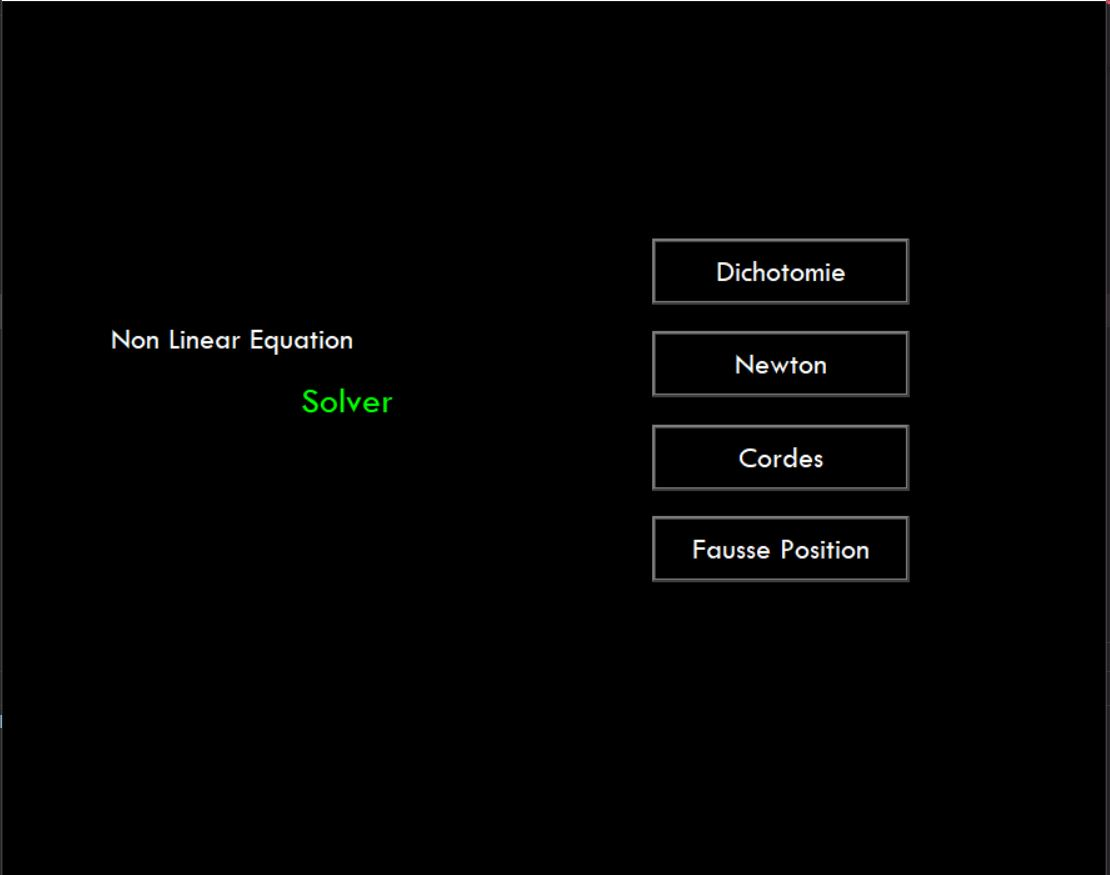
\includegraphics[width=13cm,height=8cm]{img/accueil.JPG}\\

L'interface d'accueil de notre application est constitué des quatres méthodes déjà citées afin de résoudre \\ des equations f(x)=0 et pour accéder à chaque méthode il suffit de suivre le boutton correspandant \\
à la méthode\\
Alors dans ce qui suit on va détailler chaque page dans notre interface graphique 

\subsection{Dichotomie}
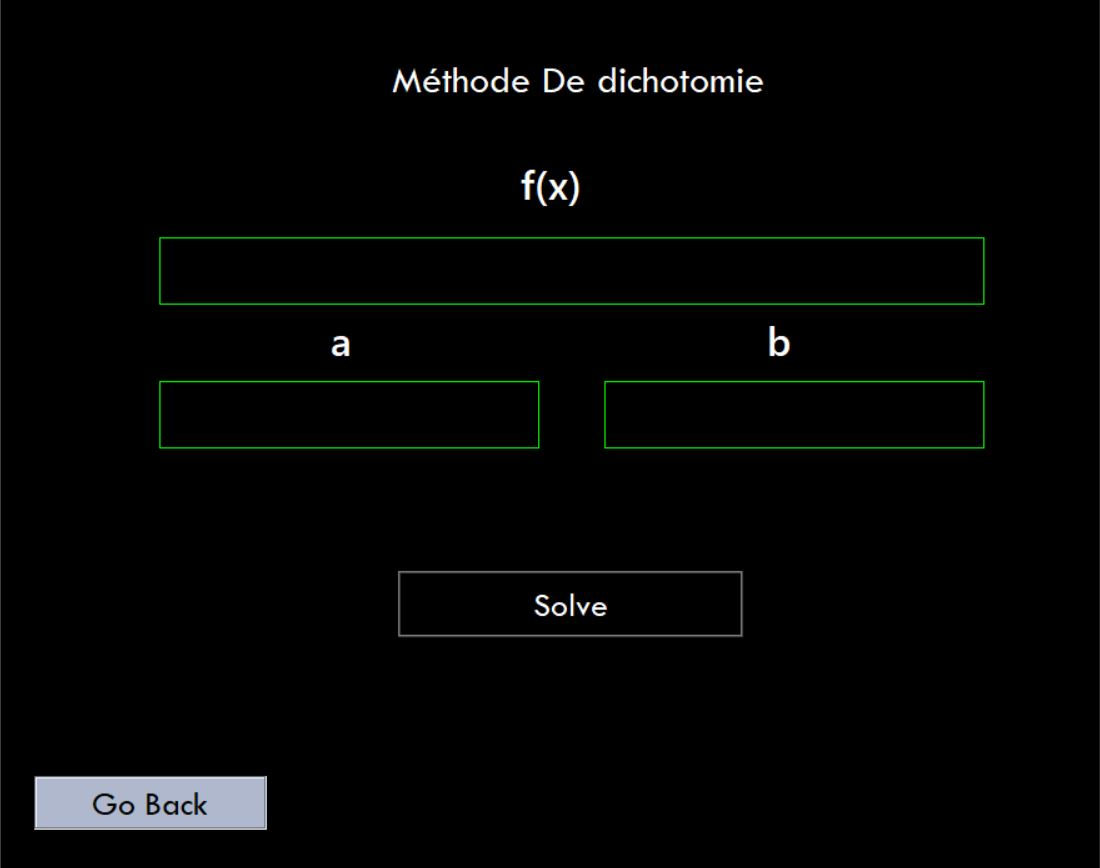
\includegraphics[width=13cm,height=8cm]{img/dicho.JPG}\\

Sur cette page on s'occupe de la méthode de dichotomie donc on prend en parametres :\\
-une fonction f\\
-un interval [a,b]

Alors si l'utilisateur de notre application rentre bien les infomations attendus et puis il clique sur le boutton solve il aura un affichage :\\
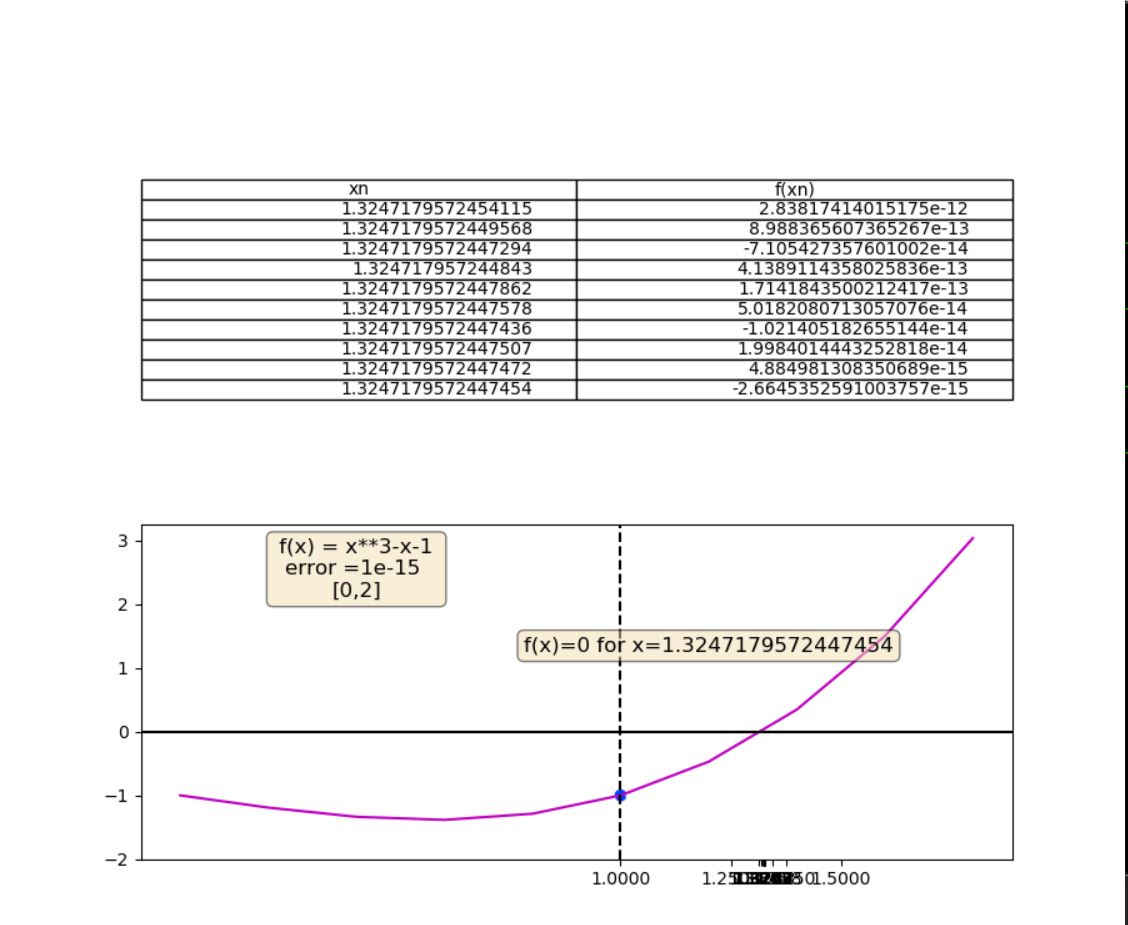
\includegraphics[width=13cm,height=7cm]{img/dicho_graph.JPG}\\

Dans la fenetre on remarque bien les informations relatives à la fonction rentrée mais aussi les résultats retournés apres éxecution de la méthode de Dichotomie \\
NB : le tableau affiche les résultats des 10 dernieres itérations de cette méthode  
\subsubsection{Convergence}
Pour la méthode de dichotomie la convergence vers la solution est graphiqueement représentés par des lignes horizontales qui se rapprochent du point cherché comme il suit : \\
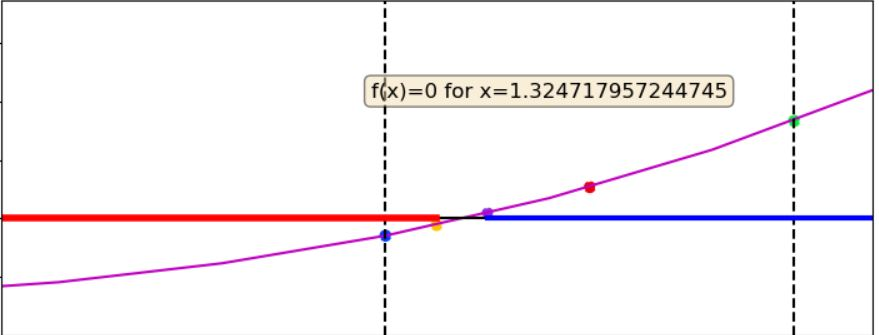
\includegraphics[width=13cm,height=7cm]{img/dicho_cv.JPG}\\


\subsection{Newton}
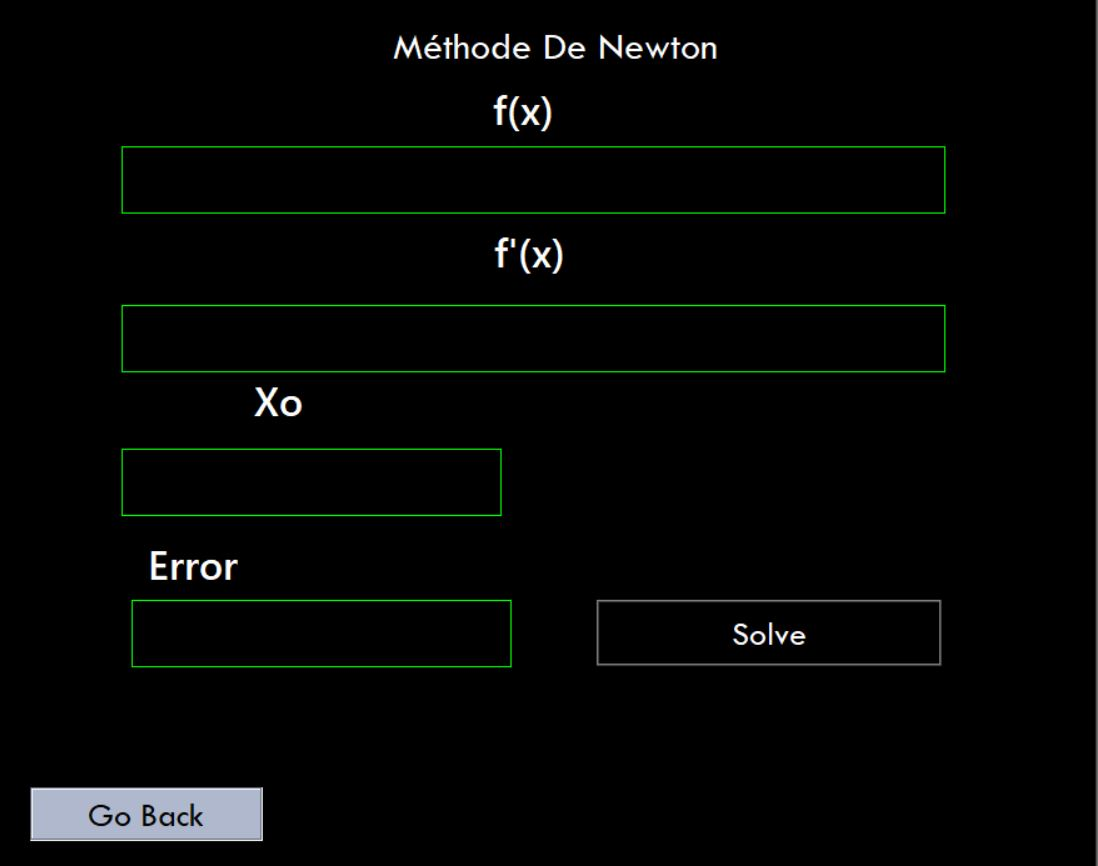
\includegraphics[width=13cm,height=7cm]{img/newton.JPG}\\

Dans cette page on résout les equations f(x)=0 à l'aide de la méthode de Newton donc on prends en arguments une fonction f et optionnellement sa dérivée et aussi un point de départ de notre récurrence  $ x_0 $
et un champ error qui indique avec quelle précision les résultats devront etre pris en compte cette valeur est initialisée à $\num{e-15}$ de base.\\
Apres rensignement des champs et cliquer sur le boutton solve une fentetre va s'afficher :\\
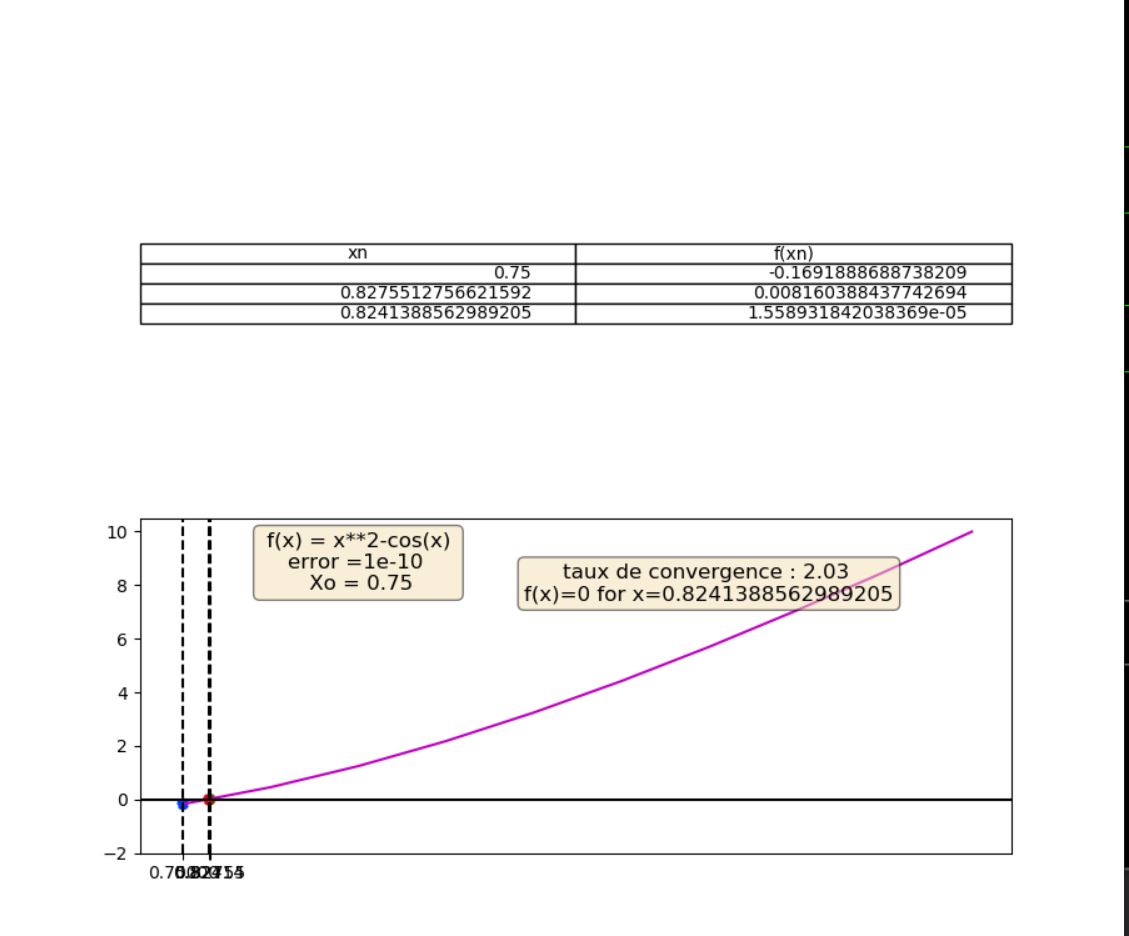
\includegraphics[width=13cm,height=7cm]{img/newton_graph.JPG}\\
avec toutes les information comme déja expliquer dans le paragraphe précédent mais cette fois çi le taux de convergence est explicitement calculé et donné avec les résultats

\subsection{Cordes}
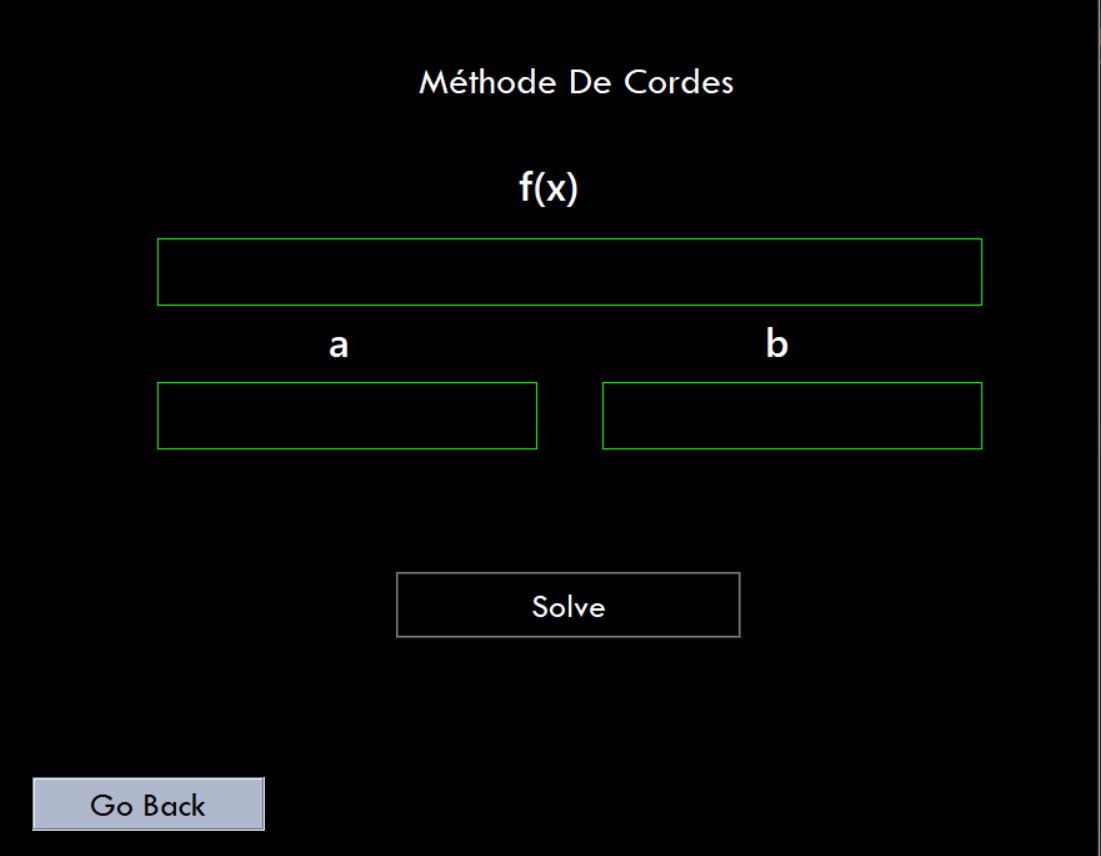
\includegraphics[width=13cm,height=7cm]{img/cordes.JPG}\\

Cette page s'occupe comme son nom l'indique de résolution des equation f(x)=0 à l'aide de la méthode des cordes elle prend en arguments une fonction f et un interval [a,b] et un clique sur le boutton solve nous donne cette fenetre :\\ 
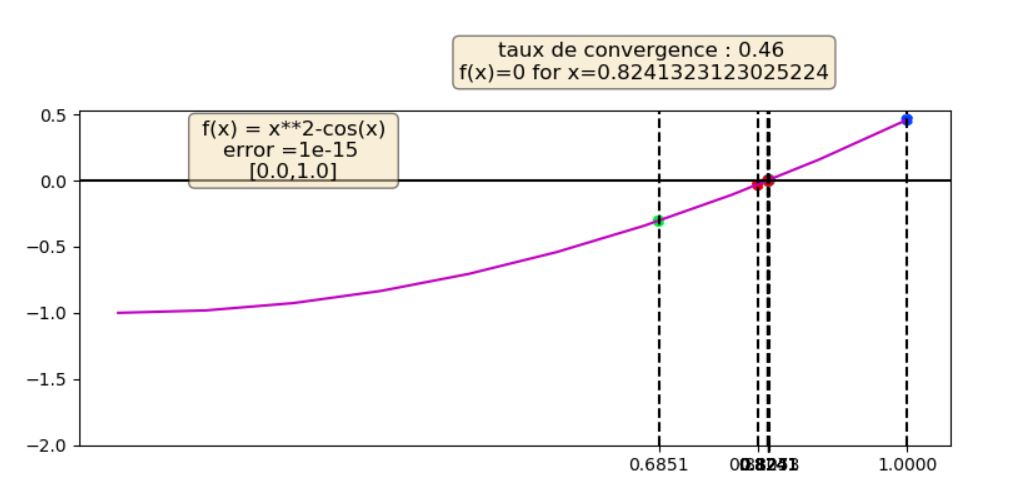
\includegraphics[width=13cm,height=7cm]{img/cordes_graph.JPG}\\

Comme bien illustré sur le graphique on nous permet de suivre la convergence de la solution volu tout en affichant le taux de convergence correspandant avec les informations nécaissaires de la fonction et l'interval.\\
\subsection{Fausse Position}
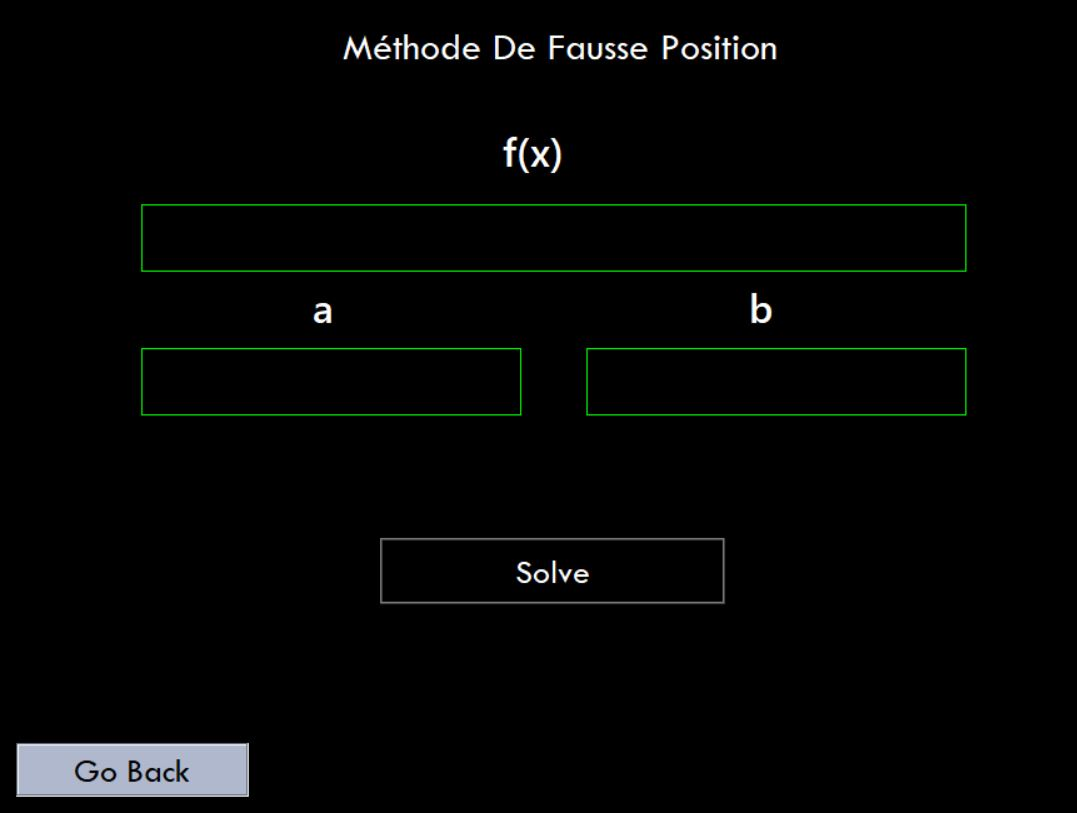
\includegraphics[width=13cm,height=7cm]{img/fausse_pos.JPG}\\

Cette page s'occupe comme son nom l'indique de résolution des equation f(x)=0 à l'aide de la méthode de fausse position elle prend en arguments une fonction f et un interval [a,b] et un clique sur le boutton solve nous donne cette fenetre : \\
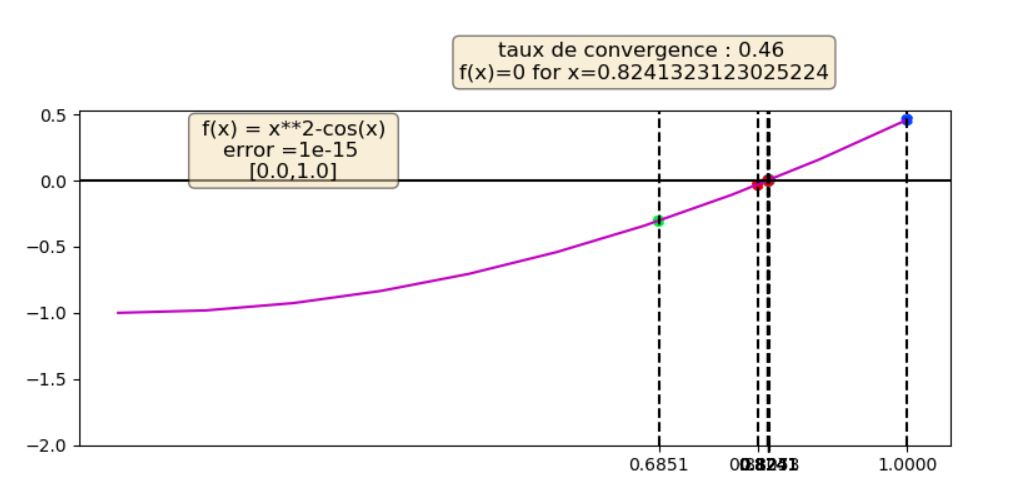
\includegraphics[width=13cm,height=7cm]{img/cordes_graph.JPG}\\

Comme bien illustré sur le graphique on nous permet de suivre la convergence de la solution volu tout en affichant le taux de convergence correspandant avec les informations nécaissaires de la fonction et l'interval.\\
\newpage
\subsection{Gestion des erreurs}
Comme déja cité dans les différentes fentetres de notre application une vérification de données tapées est nécaissaire pour le bon fonctionnement du projet alors les vérifications faites sont :

\subsubsection{Formule Erronée}
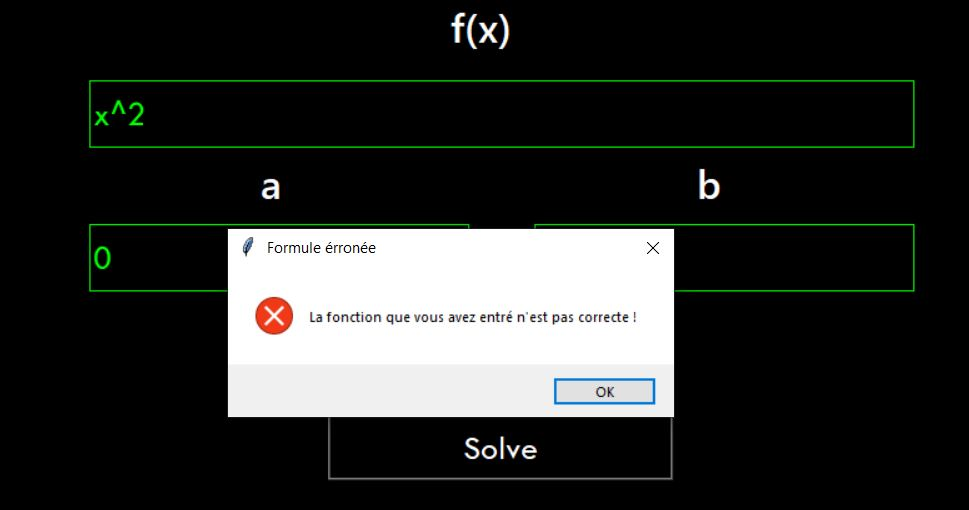
\includegraphics[width=13cm,height=6cm]{img/validation/err_fct.JPG}\\

Une formule entrée en champ dédiée est dite erronée si elle est mal exprimée au sens de Python donc toutes les formules sont supposées écrites en syntaxe de Python

\subsubsection{Monotonie}
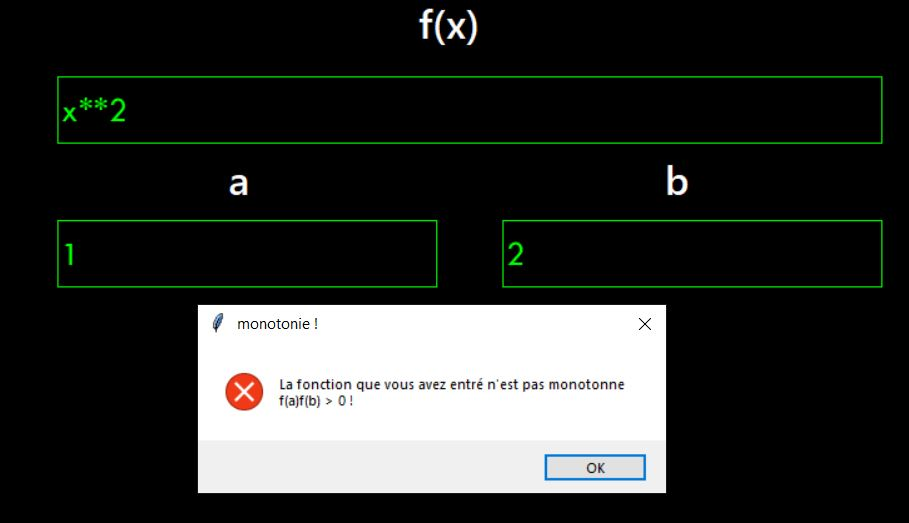
\includegraphics[width=13cm,height=6cm]{img/validation/err_fa_fb.JPG}\\

Si on rentre une fonction qui ne vérifie pas la condition des hypotheses de théoreme de valeurs intermédiaires une érreur s'affichera indiquant ce fait .

\subsubsection{Interval Erroné}
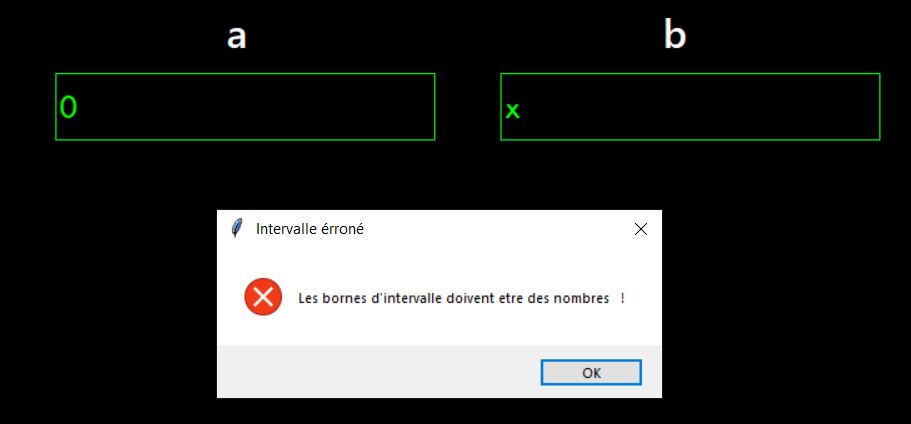
\includegraphics[width=13cm,height=5cm]{img/validation/err_interval.JPG}\\

Si on rentre un interval qui ne correspand un de ces bornes à des nombres (entiers ou floats) une érreur de type interval erroné s'affichera.

\subsubsection{Max d'itération atteint sans trouver de solution}
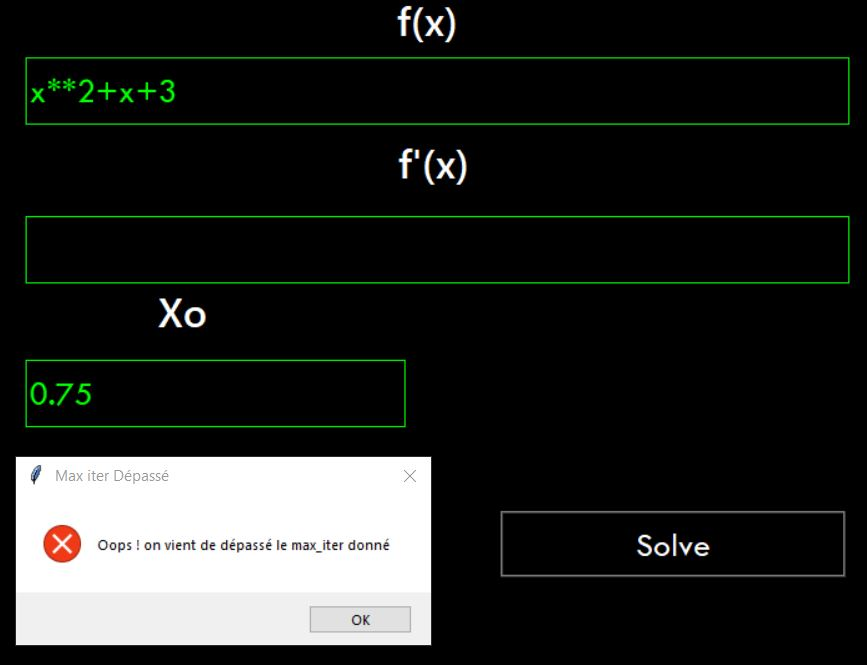
\includegraphics[width=13cm,height=8cm]{img/validation/err_max.JPG}\\

Si notre fonction n'admet pas de valeurs qui le rendent nulle dans l'interval donné et donc on atteint le maximum d'itération sans trouver de solution pour f(x)=0 alors on afficher la fentetre d'erreur ci dessous


\newpage
\section{Applications}
\newpage
\section{Conclusion}





\end{document}
